\scanpage{606}

\deleted{\unsure{To have}} \inserted{The relation} (99),
\deleted{it \unsure{suffices} to \unsure{have}} is written
\[
\tag{102}
\left\{\begin{aligned}
\deleted{\det}\sigma a&\equiv u\quad
(\mathrm{SL}(2,\widehat{\mathbb Z}))\quad\text{i.e.}\quad
\det\sigma a=\det u\quad\text{i.e. (98)}\\
\sigma a&\equiv u\quad(\deleted{4}2)
\end{aligned}\right.
\]
\deleted{\unsure{i.e.}} and this last congruence is written
\[
\tag{103}
c\equiv0\quad(\deleted{4}2)\qquad d\equiv1\quad(\deleted{4}2)
\qquad
\left(-d\equiv\mu\quad(\deleted{\unsure{4}}2)\ \text{\unsure{is a consequence of it}}
\ \text{for }\mu\equiv1\equiv-1\quad(2)\right).
\]

N.B. It is not \unsure{possible to have the} \deleted{\illegible{3} $\mu\equiv-1\ (4)$, for}
congruences \uline{mod 4}
$(\sigma a\equiv u\ (4)$, for we would have
$\mu\unsure{\equiv}-d\equiv-1\ (4)$, which is contrary to the hypothesis
(95) $\mu\equiv1\ (4)$.

\deleted{Thus (102) is \unsure{too strong}. Nevertheless, we \uline{must}
(to have (99)) have
\[
\tag{102 bis}
\sigma a\equiv u\quad(2)\qquad\text{i.e.}
\]
\[
\tag{103 bis}
c\equiv0\quad(2),\qquad d\equiv1\quad(2)
\]
(the relation $-d\equiv\mu\ (2)$ is a consequence of it, for
$\mu\equiv1\equiv-1\ (2)$). \unsure{This}}

Returning to the relation (99), we find this:

\deleted{\uuline{Proposition}} \inserted{Lemma.} Let
$c,d\in\widehat{\mathbb Z}^{\deleted{\unsure{*}}}$ satisfy
\[
\tag{104}
\mu\overset{\mathrm{dfn}}{=}-(c^2+cd+d^2)\in\widehat{\mathbb Z}^{*}
\]
\margin{\uline{N.B.} We will necessaril\textsuperscript{y} have $\mu\equiv-1\ (3)$}
\[
\tag{105}
\mu\equiv1\quad(4)\qquad
(\text{i.e. }c^2+cd+d^2\equiv-1\quad(4)).
\]
\[
\tag{106}
c\equiv0\quad(2),\qquad d\equiv1\quad(2)
\]
Let \deleted{\unsure{a c|a=}} \inserted{\unsure{d}}
\[
\tag{107}
a=\tau'(c\rho+d)=
\begin{pmatrix}-c&c+d\\d&c\end{pmatrix}
\in\mathrm{GL}(2,\widehat{\mathbb Z})
\]
(matrix with determinant $\mu$). Then we have a congruence
\[
\tag{108}
a\tau'(a)^{-1}\equiv\varepsilon\qquad
\mathrm{mod}\ \widehat{\Pi}_0\subset\mathrm{GL}(2,\widehat{\mathbb Z})
\]
\deleted{\unsure{and}} the sign $\varepsilon\in\{\pm1\}$ does not depend on the
choices made for $c,d$.

\scanpage{607}
\mspage{607}

Now is the time to calculate it! Taking up again
\[
a_0=c\rho+d\quad\in Z_\rho
\]
we will have
\[
a=\tau'a_0,\quad \tau'(a)=a_0\tau',\quad
a\tau'(a)^{-1}=\tau'a_0\tau'^{-1}a_0^{-1}=\tau'(a_0)a_0^{-1}
\]
where
\[
\left\{\begin{aligned}
\tau'(a_0)&=c\rho^{-1}+d={}^{t}a_0\\
a_0^{-1}&={}^{t}a_0/\det a_0=-\frac1\mu(c\rho^{-1}+d)
\end{aligned}\right.
\]
\margin{We \unsure{set} \inserted{for
$\unsure{u\in}\mathrm{M}_2(\widehat{\mathbb Z})$}
${}^{t}u=(\mathrm{Tr}\,u)-u$ and we have ${}^{t}\rho=\rho^{-1}$
(more generally ${}^{t}u=u^{-1}$ if $\det u=1$)}
thus
\[
a\tau'(a)^{-1}=\tau'(a_0)a_0^{-1}
=-\frac1\mu(c\rho^{-1}+d)^2
=\frac1{c^2+cd+d^2}(c\rho^{-1}+d)^2
\]
Now we have
\[
(c\rho^{-1}+d)^2
=c^2\underbrace{\rho^{-2}}_{-\rho}
+2cd\underbrace{\rho^{-1}}_{1-\rho}+d^2
=-(c^2+2cd)\rho+(2cd+d^2).
\]
Now \deleted{since}
\[
\begin{aligned}
c\equiv0\quad(2)&\Longrightarrow c^2,2cd\equiv0\quad(4)
\qquad\text{\deleted{thus}}\\
d\equiv1\quad(2)&\Longrightarrow d^2\equiv1\quad(4)
\qquad\text{thus}
\end{aligned}
\]
\deleted{
\[
a\tau'(a)^{-1}\equiv\unsure{\pm}1\quad(4)
\qquad\text{\unsure{a fortiori a}}
\]
}
\[
(\unsure{*})\qquad (c\rho^{-1}+d)^2\equiv1\quad(4)
\]
\deleted{on the other hand.}

\deleted{thus the sign $\varepsilon$ is equal to \uline{$+1$}.}

And since by hypothesis
\[
c^2+cd+d^2\equiv-1\quad(4)
\]
we will have
\[
\tag{109}
a\tau'(a)^{-1}=\frac1{c^2+cd+d^2}(c\rho^{-1}+d)^{\unsure{2}}
\equiv-1\quad(4)
\]
So we have proved, in fact

\uline{Proposition} Let $c,d\in\unsure{\mathbb Z|\widehat{\mathbb Z}}$
be such that $\xi\overset{\mathrm{dfn}}{=}c^2+\unsure{cd}+d^2
\in\widehat{\mathbb Z}^{*}$, let
\[
a=\tau'(c\rho+d)=\begin{pmatrix}-c&c+d\\d&c\end{pmatrix}
\in\mathrm{GL}(2,\widehat{\mathbb Z}),
\]
\deleted{\unsure{let us prove|let us suppose}}
\[
\deleted{(\unsure{110})}\qquad
\deleted{a\tau'(a)^{-1}}\inserted{\sigma a}
\equiv\begin{pmatrix}\xi&0\\0&1\end{pmatrix}
\quad(2)\qquad\text{i.e.}
\]
\figure{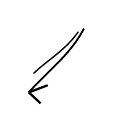
\begin{tikzpicture}[baseline]
\draw[line width=.65pt] (.8,.95) .. controls (.63,.62) and (.36,.43) .. (.1,.14);
\draw[line width=.8pt] (.1,.14)--(.34,.23) (.1,.14)--(.25,0);
\draw[line width=.5pt] (.73,.91) .. controls (.56,.67) and (.35,.56) .. (.16,.38);
\end{tikzpicture}}
\margin{\uline{N.B.} $\sigma=\begin{pmatrix}0&-1\\1&0\end{pmatrix}$}
\[
c\equiv0\quad(2),\qquad d\equiv1\quad(2).
\]

\scanpage{608}

Then we have (for $\tau'=\begin{pmatrix}-1&0\\0&1\end{pmatrix}$)
\[
a\tau'(a)^{-1}\equiv\varepsilon_2(\xi)\quad(4)
\]
(a fortiori we have the congruence mod $\widehat{\Pi}_0$).

\uline{Corollary} The extension $\mathcal E$ of $\mu\times\mu$ by $\mu$
(\unsure{84|89}), or of $\mu$ by $\mathcal E''\simeq\mathbb Z/4\mathbb Z$, is noncommutative.
\margin{$\big|$}

But here is a way of seeing it without calculation. If the extension were commutative,
\deleted{it} \inserted{its isomorphism class} would be given by an
$\unsure{\mathrm{Ext}_{\mathbb Z}|\mathrm{Ext}^1_{\mathbb Z}}$
(or an $\mathrm{Ext}^{\unsure{1|?}}_{\mathbb Z/4\mathbb Z}$).
Now the functor $\unsure{\mathrm{Ext}|\mathrm{Ext}^1}(-,\mu)$ is additive. Since the restriction of
the extension to the subgroups $\mathcal E'/\mu$ and $\mathcal E'''/\mu$ of
$\mu\times\mu$ is trivial, and $\mu\times\mu$ is
the direct sum of these subgroups (which are resp. $1\times\mu$ and the
diagonal subgroup), it would follow that the extension would be
trivial, but we have seen that this is not the case.

\deleted{\unsure{In|And}} \unsure{The} structure of the group $\mathcal E$
is readily made explicit, for example in its \unsure{capacity} as an extension of
$\mathcal E/\mathcal E''\simeq\mu$ by
$\mathcal E''\simeq\mathbb Z/4\mathbb Z$. \deleted{Let}
Let us choose any element of $\mathcal E-\mathcal E''$, it is
of order 2 (the only elements of order 4 being in $\mathcal E''$) so
that we have

\scanpage{609}
\mspage{608}

\[
\tag{110}
\mathcal E\simeq\{1,x\}\mathbin{.}\mathcal E''
\qquad\left(\tfrac12\ \text{direct}\right)
\]
Let us note that if $x$ operated trivially on $\mathcal E''$,
\deleted{i.e.} if $\mathcal E$ were isomorphic to the product, then for an
element \inserted{$u$ of $\mathcal E''$} of order 4,
$x.u$ would be of order \unsure{4|8}, which is absurd (third proof of the fact
that \inserted{$\mathcal E/\mathcal E''\simeq$} $\mu$ operates nontrivially
on $\mathcal E''$). Now from the mere fact that the operation of $\{1,x\}$ on
$\mathcal E''$ is nontrivial\unsure{.}, it is known, and
\inserted{the structure of} $\mathcal E$ is determined -- in fact we have
\[
\tag{\unsure{111|110}}
\mathcal E\simeq\mathbb D_4
\]
There is a preferred choice of $x$, by taking for $x$ the elemen\unsure{t}
\[
\tag{112}
\left\{\begin{aligned}
\tau_{\mathcal E}&\overset{\mathrm{dfn}}{=}
\tau_{\unsure{S_0\Gamma}}\ \mathrm{mod}\ S_0^{\Pi}\Gamma^0,
\quad\text{where of course}\\
\tau_{S_0\Gamma}&=(\tau,\tau',\tau),
\end{aligned}\right.
\]
so that we have a canonical representation
\[
\tag{113}
\mathcal E\simeq\{1,\tau_{\mathcal E}\}\mathbin{.}
\mathcal E''
\qquad\text{product }\tfrac12\text{ direct}
\]
\margin{$\mathcal E''\simeq\mathbb Z/4\mathbb Z$\quad
$\tau_{\mathcal E}(u)=u^{-1}$ for $u\in\mathcal E''$.}

The homomorphism $\mathcal E\to\mu\times\mu$ is recovered from its restrictions to the
two factors
\[
\tag{114}
\diagram{\begin{tikzcd}[column sep=large,row sep=large]
\mu\simeq\{1,\tau_{\mathcal E}\}\arrow[r]&\mu\times\mu&
\tau_{\mathcal E}\arrow[r,mapsto]&(-1,-1)\quad\text{(diagonal homomorphism)}\\
\mathcal E''\arrow[r]&\unsure{\mu\times\{1\}}\arrow[r,hook]&\mu\times\mu&
\end{tikzcd}}
\]
the unique nontrivial homomorphism $\mathcal E''\to\mu$ deduced from the isomorphism
\[
\diagram{\begin{tikzcd}
\mathcal E''_2\overset{\mathrm{dfn}}{=}
\unsure{\mathcal E''/2\mathcal E''|\mathcal E''/{}_{2}\mathcal E''}
\arrow[r,"\sim"]&\mu
\end{tikzcd}}
\]

\scanpage{610}

The fact that $\mathcal E$ is not commutative is also expressed by the fact
that the canonical homomorphism
\[
\tag{115}
\diagram{\begin{tikzcd}
\mathcal E_{\mathrm{ab}}\arrow[r,"\sim"]&\mu\times\mu
\end{tikzcd}}
\]
is an isomorphism, i.e. that the kernel subgroup $\mu$ of
$\unsure{\mathcal E_{\mathrm{ab}}|\mathcal E}\to\mu\times\mu$ is also
the commutator subgroup.

We have seen that the extension $\mathcal E$ of $\mu\times\mu$ by $\mu$ is not
split, but what about its inverse image, the extension
$S_0^{\Pi}\Gamma^!$ of $Z^!\simeq\mathcal M[0]$ by $\mu$? A priori,
we only know that there is no splitting of this extension which
extends the canonical splitting $A$ we have over
\[
Z^0=\mathrm{Ker}\left(\diagram{\begin{tikzcd}
Z^!\arrow[r,"(\varepsilon_3,\varepsilon_2)"]&\mu\times\mu
\end{tikzcd}}\right).
\]
I presume that even $S_0^{\Pi}\Gamma''$, an extension of
$Z^{!\unsure{\prime\prime}}$ by $\mu$, is nontrivial, and
even the extension it induces on the subgroup
\[
\Gamma'_{\mathbb Q}=\Gamma_{\mathbb Q}\cap
\underbrace{\Gamma_{\mathbb Q}^{\prime\sim}}_{\substack{\wr\\\mathcal M(0)'}}
\subset\mathcal M^{\unsure{\xi|*}}(0)\subset\mathcal M^![0]=Z^!.
\]
It would be interesting to identify, \deleted{the ext}
more precisely, the extension over $\Gamma_{\mathbb Q}$, which it induces, which
corresponds to a canonical element
\[
\tag{115}
c\in H^{\unsure{2}}(\mathrm{Spec}\,\mathbb Q,\mu_2)\subset\mathrm{Br}(\mathbb Q)
\]

\scanpage{611}
\mspage{609}

Unless I am mistaken we will have
\[
\tag{115}
c=\underset{\text{(cup-product)}}{\xi'\xi''},
\quad\text{where}\quad
\xi',\xi''\in
H^2(\mathbb Q,\unsure{\mu_2})
\]
are the elements which describe respectively the extensions
$\mathbb Q(\sqrt[3]{1})=\mathbb Q(\sqrt{-3})$, and
$\mathbb Q(\sqrt{3})$ --- both contained, as well as
$\mathbb Q(\sqrt{-1})=\mathbb Q(i)$, in the biquadratic extension
$\mathbb Q\bigl(\underset{\substack{\Vert\\\sqrt[2]{-1}}}{i},
\underset{\substack{\Vert\\\sqrt[3]{1}}}{j}\bigr)
=\mathbb Q(\sqrt[12]{1})$, the field of
$12^{\text{th}}$ roots of unity (whose Galois group is
$(\mathbb Z/12\mathbb Z)^*\simeq(\mathbb Z/3\mathbb Z)^*\times
(\mathbb Z/4\mathbb Z)^*\simeq\mu\times\mu$).

It must be trivial --- when one \unsure{knows} a little of the foundations ---
that $c$ thus made explicit is $\ne0$, and is not
\unsure{split} either on passing to $\mathbb Q(i)$, the third rogue.

\figure{\begin{tikzpicture}\draw (0,0)--(2,0);\end{tikzpicture}}

Let us now consider the central $\mu$-\unsure{grouping}
\margin{\uline{N.B.} $Z\simeq\mathcal M[0]$, $\gamma\simeq\widetilde{\Gamma}_{\mathbb Q}$}
\[
\tag{116}
\diagram{\begin{tikzcd}[column sep=large]
\mu \arrow[r,hook,"i_{\rho,\mu}"] &
S_0\Gamma^!_{\rho,\sigma}
=Z^!_{\rho,\sigma}\times_\gamma N^*_\rho\times_\gamma N^*_\sigma\\
\varepsilon \arrow[r,mapsto] & (1,\varepsilon,1)
\end{tikzcd}}
\]
with values in
\[
\operatorname{Ker}(S_0\Gamma^!_{\rho,\sigma}\longrightarrow
Z^!_{\rho,\sigma})\simeq L_\rho\times L_\sigma,
\]
we thus have a canonical lifting homomorphism
\[
\tag{117}
\diagram{\begin{tikzcd}[column sep=large]
\mathcal M^![0]\simeq Z^!_{\rho,\sigma}
\simeq S_0^\Pi\Gamma^!_{\rho,\sigma}/\mu
\arrow[r] & S_0\Gamma^!_{\rho,\sigma}/i_{\rho,\mu}(\mu),
\end{tikzcd}}
\]

\scanpage{612}

which is made explicit in terms \unsure{\deleted{of the}|of the} two
fundamental canonical homomorphisms
\margin{This deserves to be made explicit in a summarizing theorem $\ldots$}
\[
\tag{118}
\diagram{\begin{tikzcd}[column sep=large,row sep=small]
Z^!_{\rho,\sigma} \arrow[r,"\uline{a}"]
\arrow[d,phantom,"\simeq"{description,sloped}] & N^*_\rho/\mu,
& Z^!_{\rho,\sigma} \arrow[r,"\uline{b}"] & N^*_\sigma\\
\mathcal M[0] \arrow[d,phantom,"\simeq"{description,sloped}] &&&\\
\widetilde{\Gamma}_{\mathbb Q}\mathbin{.}L_0^{\unsure{\Pi}} &&&
\end{tikzcd}}
\]
where, I recall
\[
\tag{119}
\left\{\begin{array}{l}
N^*_\rho\subset\mathcal M=\widetilde N_{1,1}\simeq
\widetilde\Gamma_{\mathbb Q}\mathbin{.}
\underbrace{\mathcal G^+}_{\mathrm{SL}(2,\mathbb Z)^\wedge}\\
\Vert\\
\{u\in\mathcal M\mid
u(\rho)=\deleted{\text{\unsure{fixes the group}}}\rho^{\varepsilon_3(u)}\}\\[1ex]
\deleted{\unsure{\{}}N^*_\sigma\subset\mathcal M\\
\Vert\\
\{u\in\mathcal M\mid u(\sigma)=\sigma^{\varepsilon_2(u)}
\ (=\varepsilon_2(u)\sigma)\}.
\end{array}\right.
\]

The maps $\uline{a},\uline{b}$ are given by the formulas (cf. 51)
\[
\tag{120}
\left\{\begin{array}{ll}
\uline{a}(u)=a=\varepsilon_3[\tau']\alpha^{-1}u,
& \uline{b}(u)=b=\beta^{-1}u\quad\text{i.e.}\\
\alpha=ua^{-1}\varepsilon_3[\tau'],&\beta=ub^{-1}
\end{array}\right.
\]
where $\alpha\in\widehat\Pi_{0\tau}$, $\beta\in\widehat\Pi_0$
are characterized by
\[
\tag{121}
u(\rho)=\operatorname{int}(\alpha)(\rho),\quad
u(\sigma)=\varepsilon_2(\sigma)\operatorname{int}(\beta)(\sigma).
\]
The quantities \deleted{\unsure{$a,$}}
$a=\uline{a}(u)\inserted{\in N^*_\rho/\mu}$,
$b=\uline{b}(u)\inserted{\in N^*_\sigma}$ are characterized in terms of
$u\in Z^!$ (only up to a sign) by the congruences
\[
\tag{122}
u\equiv b\quad(\widehat\Pi_0),\qquad
u\equiv\varepsilon_3[\sigma]a\quad(\widehat\Pi),
\]
which imply a fortiori (reducing mod $\mathcal G^{+\wedge}$),
that we have commutativity \unsure{of the|of},